	
	\subsection{Главные аффинные окрестности}\hypertarget{bilet_7}{}

	 \begin{definition} 
	 	\emph{Главным открытыми множествами (или, аффинными окрестнстями) в $\AA^n$} назвают множества вида 
	 	\[
	 		D(f) \eqdef \AA^n \setminus Z(f),
	 	\]
	 	где $f$~--- некоторый многочлен из $\bk[x_1, \ldots, x_n]$.

	 	Пусть $X$~--- аффинное многообразие, $\overline{f} \in A(X) = \Bbbk[x_1, \ldots, x_n]/I(X)$, тогда определим
	 \[
	 	D(\overline{f}) \eqdef D(f) \cap X = X \setminus Z\lr*{\overline{f}}. 
	 \]
	 \end{definition}


	 \begin{remark}
	 	Ясно, что если $f = 1$, то $D(f) = \AA^n$, откуда $D(\overline{f}) = X$.
	 \end{remark}

	 Для краткости обозначим $A = A(X)$ и рассмотрим  главную локализацию 
	 \[
	 	A_{\overline{f}} = S^{-1}A, \text{ где } S = \{ \overline{f}^n \ \vert \ n \in \N \}. 
	 \]
	 
	 \begin{remark}
	 	Отметим, что возможен случай, когда $A_{\overline{f}} = 0$, но тогда $\exists k\colon \overline{f}^k = 0$, а так как $I(X)$~--- радикальный идеал, это равносильно тому, что $\overline{f} = 0$, что равносильно тому, что $f \in I(X)$, т.е.
	 	\[
	 		D(\overline{f}) = X \setminus Z(\overline{f}) = \varnothing. 
	 	\]
	 \end{remark}

	 В случае, когда $D(\overline{f}) \neq \varnothing$, мы полуачем гомоморфизм колец 
	 \[
	 	A_{\overline{f}} \to \cO(D(\overline{f})), \quad  \frac{\overline{a}}{\overline{f}^k} \mapsto \text{ функция } \frac{\overline{a}}{\overline{f}^k}
	 \]

	 \begin{itemize}
	 	\item Этот гомоморфизм инъективен: 
	 	\[
	 	\frac{\overline{a}}{\overline{f}^k}\bigg\vert_{D\lr*{\overline{f}}} = 0 \implies \overline{a}\vert_{D\lr*{\overline{f}}} = 0 \implies \overline{a}\cdot \overline{f}\vert_{X} = 0 \implies af \in I(X) \implies \overline{a} \overline{f} = 0 \in A(X),
	 \]
	 откуда $\overline{a}/\overline{f}^k = 0$ в локализации $A(X)_{\overline{f}}$. 

	 	\item Кроме того, он сюръективен. Пусть $r \in \cO\lr*{D\lr*{\overline{f}}}$, тогда 
	 	\[
	 		x \in D\lr*{\overline{f}} \quad \exists \text{ окрестность } U_x \ni x , \ \overline{g}_x, \overline{h}_x \in A(X)\colon  r \overline{h}_x = \overline{g}_x \text{ на } U_x
	 	\]
	 	и $h_x$ не имеет нулей в $U_x$. 

	 Выбирая многочлен $s_x \in A(X)$, не равный нулю в точке $x$, но обращающийся в ноль на дополнении, мы можем полагать, что наше равенство выполнено на всём $X$ (см. доказательство теоремы~\ref{O(X) = A(X)}). Не умаляя общности, будем считать так изначально. Заметим, что 
	 \[
	   	Z\lr*{\sum_{x \in D\lr*{\overline{f}}} (h_x) + I(X)} \subset Z(f),
     \]  
     так как если $y \in \sum_{x \in D\lr*{\overline{f}}} (h_x) + I(X)$, то $y \in X \setminus D(\overline{f}) = X \cap Z(f)$. Тогда 

     \[
     	\sqrt{(f)} \subset \sqrt{\sum_{x \in D\lr*{\overline{f}}} (h_x) + I(X)} \implies f^m \in \sum_{x \in D\lr*{\overline{f}}} (h_x) + I(X) \implies \overline{f}^m \in \sum_{x \in D\lr*{\overline{f}}} (h_x) 
     \]

     Значит, мы можем представить $\overline{f}^m$ в виде 
     \[
     	\overline{f}^m = \sum_{i = 1}^{k} \overline{h_{x_i}} \overline{\ell_i}, \quad x_i \in D\lr*{\overline{f}}.
     \]
     Но тогда, домножая это равенство на $r$ мы получаем 
     \[
     	\overline{f}^m r = \sum_{i = 1}^{k} \overline{g_{x_i}} \overline{\ell_{x_i}} \implies r = \frac{\overline{a}}{\overline{f}^m} \in A_{\overline{f}}. 
     \]
	 
	 \end{itemize}
	
 	
   Таким образом, мы доказали такое предложение 

	\begin{statement}\label{A_f = O(D(f))} 
		$A(X)_{\overline{f}} \cong \cO(D\lr*{\overline{f}})$.
	\end{statement}

	Полезно также рассмотреть алтернативное доказательство этого факта. 

	\begin{proof}[Альтернативное доказательство предложения~\ref{A_f = O(D(f))}]
		Рассмотрим отображение 
		\[
			A_{\overline{f}} \xrightarrow{\sim} A[t]/\lr*{\overline{f}t - 1}, \quad \frac{a}{\overline{f}^k} \mapsto \overline{a} t^k.
		\]
		Легко видеть, что это изоморфизм. Кроме того, 
	   \[
	    	A = \Bbbk[x_1, \ldots, x_n]/I(X) \implies A[t]/\lr*{\overline{f}t - 1} \cong \Bbbk[x_1, \ldots, x_n, t]/\lr*{I(x), \overline{f}t - 1},
	    \] 
	    откуда видно, что $A_{\overline{f}}$~--- это координатное кольцо многообразия
	    \[
	    	Y = \{ (x_1, \ldots, x_n, t) \in \AA_{\Bbbk}^{n + 1} \ \vert \ (x_1, \ldots, x_n) \in X, \quad f(x_1, \ldots, x_n) t - 1 = 0 \}. 
	    \]
	    Рассмотрим коммутативную диаграмму: 
	    \begin{center}
	    	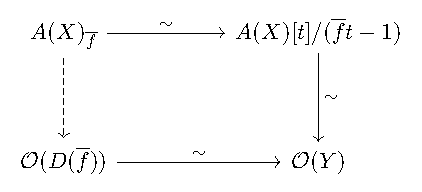
\includegraphics{lectures/5/pictures/cd_1.pdf}
	    \end{center}

	    Нижняя горизонтальная стрелка получается из того, что $Y \xrightarrow{\sim} D\lr*{\overline{f}}$ посредством (взаимнообратных) отображений 
	    \[ 
	    	(x_1, \ldots, x_n, t) \mapsto (x_1, \ldots, x_n), \quad (x_1, \ldots, x_n) \mapsto (x_1, \ldots, x_n, 1/f(x_1, \ldots, x_n))
	    \]

	    Так как горизонтальные и правая вертикальная стрелка~--- изоморфизмы, левая вертикальная стрелка~--- тоже изоморфизм. 


	\end{proof}
	   
	  \subsection{Эквивалентные определения размерности неприводимого аффинного многообразия}

	    \begin{statement} 
	    	Пусть $X$~--- неприводимое квазиаффиное многообразие, $U \subset X$~--- открытое подмножество. Тогда $\dim{U} = \dim{X}$.
	    \end{statement}
	    \begin{proof}
	    	\bf{\RNum{1}.} Пусть $X$~--- аффинное. Тогда так как $U$ открытое, 

	    	\[
	    		U = X \setminus Z(\overline{f_1}, \ldots, \overline{f_n}) \supset X \setminus Z(\overline{f_j}) = D\lr*{\overline{f_j}} \implies D\lr*{\overline{f_j}} \subset U \subset X \implies 
	    	\]
	    	\[
	    		\implies \dim{D\lr*{\overline{f_j}}} \le \dim{U} \le \dim{X}.	
	    	\]	
	    	Но, как мы знаем из предложения~\ref{A_f = O(D(f))} и теоремы~\ref{dim_tr_deg}, $\dim{D\lr*{\overline{f_j}}} = \dim{A(X)_{\overline{f_j}}} = \Trdeg{\Frac{A(X)_{\overline{f_j}}}}$. Теперь заметим, что 
	    	\[
	    	 	\Trdeg{\Frac{A(X)_{\overline{f_j}}}} = \Trdeg{\Frac{A(X)}} = \dim{X}, 
	    	 \] 
	    	 откуда мы заключаем, что $\dim{U} = \dim{X}$.
	    		

	    	\bf{\RNum{2}.} Пусть $X$ квазиаффинное. Тогда $U \subset X \subset \overline{X}$ и $\overline{X}$~--- аффинное. Тогда, так как $U$~--- открытое подмножество $\overline{X}$, по пункту $\RNum{1}$ мы имеем 
	    	\[
	    		\dim{U} = \dim{\overline{X}}.
	    	\]
	    	С другой стороны, $\dim{U} \le \dim{X} \le \dim{\overline{X}}$, откуда мы получили нужное. 
	    \end{proof}

	    \begin{definition} 
	    	Пусть $X$~--- квазиаффинное многообразие. Тогда $\dim{X}$~---  наибольшая из размерностей его неприводимых компонент. 
	    \end{definition}

	    \subsection{Прямое произведение многообразий и его первые приложения}

	    
    	Пусть $X \subset \AA^m, \ Y \subset \AA^n$~--- аффинные многообразия. Пусть $X = Z(f_1, \ldots, f_k), \ Y = Z(g_1, \ldots, g_{\ell})$, то 
    	\[
    		X \times Y = \{ (x_1, \ldots, x_m, y_1, \ldots, y_n) \vert f_i(x_1, \ldots, x_m) = 0, \ g_j(y_1, \ldots, y_n) = 0 \ \forall i, j \}.
    	\]

    	То есть, прямое произведение естественно снабжается структурой аффинного многообразия в $\AA^{m \times n}$. Позже мы докажем, что это произведение в категорном смысле. 

    	Также видно, что если $X$ и $Y$~--- квазиаффинные, то их прямое произведение тоже квазиаффинное. 

    	\begin{statement}\label{direct_product_of_irr} \hypertarget{bilet_13}{} 
    		Пусть $X \subset \AA^m, \ Y \subset \AA^n$~--- неприводимые аффинные многообразия, то $X \times Y$~--- неприводимое аффинное многообразие в $\AA^{m} \times \AA^{n}$.
    	\end{statement}
	    	\begin{proof}
	    		Предположим противное, то есть, что 
	    		\[
	    			X \times Y = Z_1 \cup Z_2, \quad Z_i \neq X \times Y. 
	    		\]
	    		Ясно, что $\forall x \in X \quad x \times Y \cong Y$~--- неприводимое, тогда $x \times Y \subset Z_1$ или $x \times Y \subset Z_2$. Но тогда 
	    		\[
	    			X = X_1 \cup X_2, \quad X_j = \{ x \ \vert \ x \times Y \subset Z_j \}.
	    		\]

	    		Покажем, что множества $X_1$ и $X_2$ замкнутые. Для этого достаточно заметить, что 
	    		\[
	    			X_1 = \bigcap_{y \in X} X_{y}, \text{ где } X_y = \{ x \in X \ \vert \ (x, y) \in Z_1 \},
	    		\]
	    		а $X_y$~--- замкнуты, так как если $Z_1 = Z(f_1(x, y), \ldots, f_k(x, y))$, то 
	    		\[
	    			X_{\widetilde{y}} = Z(f_1(x, \widetilde{y}), \ldots, f_k(x, \widetilde{y})).
	    		\]
	    		Тогда мы приходим к противоречию, так как из неприводимости $X$ следует, что $X \subset X_1$ или $X \subset X_2$, откуда $X \times Y = Z_1$ или $X \times Y = Z_2$ (что противоречит нашему предположению). 

		\end{proof}
	   \begin{statement}\hypertarget{bilet_14}{} 
	    	Пусть $X, Y$~--- неприводимые аффинные многообразия. Тогда $\dim{(X \times Y)} = \dim{X} + \dim{Y}$.
    	\end{statement} 	
    	\begin{proof}
    		Пусть $\dim{X} = r, \ \dim{Y} = s$. Поле функций $\Bbbk(X)$ порождается ровно  $r$ алгебраически независимыми координатными функциями $u_1, \ldots, u_r$. Аналогично, $\Bbbk(Y)$ порождается координатныими функциями $v_1, \ldots, v_s$ и они алгебраически независимы. Тогда совершенно ясно, что 
	\[
		\dim{(X \times Y)} = \mathrm{trdeg}\lr*{\Bbbk(X \times Y)} \le r + s.
	\]

	Остаётся показать, что система $(u_1, \ldots, u_r, v_1, \ldots, v_s)$ будет алгебраически независимой в $\Bbbk(X \times Y)$. 

	Предположим, что 
	\[
		\sum f_{i_1 i_2 \ldots i_r}(v_1, \ldots, v_s) u_1^{i_1} \cdot \ldots \cdot u_{r}^{i_r} = 0.
	\]

	Подставляя $a_i \in \Bbbk$, мы получаем полиномиальное соотношение на $u_i:$

	\[
		\sum f_{i_1 i_2 \ldots i_r}(a_1, \ldots, a_s) u_1^{i_1} \cdot \ldots \cdot u_{r}^{i_r} = 0,
	\]
	а так как $u_i$ алгебраически независимы, отсюда следует, что $f_{i_1 \ldots i_r}(a_1, \ldots, a_s) = 0$. По произвольности набора  $a_1, \ldots, a_s$, мы получаем, что $f_{i_1 i_2 \ldots i_r}(v_1, \ldots v_s) = 0$, но так как $v_i$ алгебраически независимы, отсюда следует, что $f_{i_1 \ldots i_r} = 0$, что и требовалось. 
    	\end{proof}

    	\begin{remark}
    		Здесь мы по существу использовали, что для аффинных $\bk(X) = \Frac{A(X)}$.
    	\end{remark}

    Обсудим, что происходит в случае приводимых многообразий. Если 
	\[
		X = \bigcup_{i} X_{i}, Y = \bigcup_{j} Y_{j} \quad X_{i}, Y_{j} \text{~--- неприводимые},
 	\]
 	то $\dim{X} = \max{\dim{X_i}}$, а $\dim{Y} = \max{\dim{Y_j}}$. Тогда у нас есть разложение $X \times Y$ в неприводимые:
 	\[
 		X \times Y = \bigcup X_i \times Y_j 
 	\]

 	Таким образом, мы получили, что 

 	\begin{statement} 
 		Пусть $X, Y$~--- многообразия, тогда $\dim(X \times Y) = \dim{X} + \dim{Y}$. 
 	\end{statement}

	    \begin{theorem} \hypertarget{bilet_17}{}
	    	Пусть $Y, Z \subset \AA_{\Bbbk}^n$~--- неприводимые аффинные многообразия, $\dim{Y} = r, \ \dim{Z} = s$. Тогда любая компонента $Y \cap Z$ имеет размерность $\ge r + s - n$.
	    \end{theorem}
	    \begin{proof}
	    	Рассмотрим диагональное вложение 
	    	\[
	    		\Delta\colon \AA^n \to \AA^{n} \times \AA^{n} = \AA^{2n}, \ x \mapsto (x, x). 
	    	\]

	    	Образ $\Delta(\AA^n)$ замкнут в $\AA^{2n}$, так как он задаётся вот такой системой уравнений: 
	    	\begin{equation}
	    		\begin{cases} y_1 = y_{n + 1} \\ y_2 = y_{n + 2} \\ \vdots \\ y_{n} = y_{2n} \end{cases} \label{Delta(A^n)}
	    	\end{equation}

	    	Заметим, что имеет место изоморфизм 
	    	\[
	    		Y \cap Z \xrightarrow{\sim} \Delta\lr*{\AA^n} \cap (Y \times Z).
	    	\]
	    	Так как при изоморфизме неприводимые компоненты переходят в неприводимые компоненты, размерности неприводимых компонент левой и правой частей равны. Заметим, что $\Delta(\AA^n)$~--- пересечение $n$ гиперповерхностей (как видно из~\ref{Delta(A^n)}. Тоогда, пользуясь теоремой~\ref{dim{X} - m} (и тем фактом, что $\dim{Y \times Z} = r + s$), мы получаем нужное. 

	    \end{proof}

	    Заметим, что в процессе доказательства мы установили, что $D(\overline{f})$ изоморфно аффинному подмногообразию в $\AA^{n + 1}$.

    	\begin{exercise}
			Если $X, Y$~--- аффинные, то $A(X \times Y) \cong A(X) \otimes_{\Bbbk} A(Y)$.    
    	\end{exercise}
    	\begin{remark}
    		Над алгебраически замкнутым полем тензорное произведение целостных конечно порожденных алгебра~--- целостная конечно порожденная алгебра. Если поле не алгебраически замкнутое, то это не обязательно так. 
    	\end{remark}

    	





